%%% Hlavní soubor. Zde se definují základní parametry a odkazuje se na ostatní části. %%%

%% Verze pro jednostranný tisk:
% Okraje: levý 40mm, pravý 25mm, horní a dolní 25mm
% (ale pozor, LaTeX si sám přidává 1in)
\documentclass[12pt,a4paper]{report}
\setlength\textwidth{145mm}
\setlength\textheight{247mm}
\setlength\oddsidemargin{15mm}
\setlength\evensidemargin{15mm}
\setlength\topmargin{0mm}
\setlength\headsep{0mm}
\setlength\headheight{0mm}
% \openright zařídí, aby následující text začínal na pravé straně knihy
\let\openright=\clearpage

%% Pokud tiskneme oboustranně:
% \documentclass[12pt,a4paper,twoside,openright]{report}
% \setlength\textwidth{145mm}
% \setlength\textheight{247mm}
% \setlength\oddsidemargin{15mm}
% \setlength\evensidemargin{0mm}
% \setlength\topmargin{0mm}
% \setlength\headsep{0mm}
% \setlength\headheight{0mm}
% \let\openright=\cleardoublepage

%% Použité kódování znaků: obvykle latin2, cp1250 nebo utf8:
\usepackage[utf8]{inputenc}

%% Ostatní balíčky
\usepackage{graphicx}
\usepackage{amsthm}

%% Balíček hyperref, kterým jdou vyrábět klikací odkazy v PDF,
%% ale hlavně ho používáme k uložení metadat do PDF (včetně obsahu).
%% POZOR, nezapomeňte vyplnit jméno práce a autora.
\usepackage[ps2pdf,unicode]{hyperref}   % Musí být za všemi ostatními balíčky
\hypersetup{pdftitle=Název práce}
\hypersetup{pdfauthor=Jméno Příjmení}

%%% Drobné úpravy stylu

% Tato makra přesvědčují mírně ošklivým trikem LaTeX, aby hlavičky kapitol
% sázel příčetněji a nevynechával nad nimi spoustu místa. Směle ignorujte.
\makeatletter
\def\@makechapterhead#1{
  {\parindent \z@ \raggedright \normalfont
   \Huge\bfseries \thechapter. #1
   \par\nobreak
   \vskip 20\p@
}}
\def\@makeschapterhead#1{
  {\parindent \z@ \raggedright \normalfont
   \Huge\bfseries #1
   \par\nobreak
   \vskip 20\p@
}}
\makeatother

% Toto makro definuje kapitolu, která není očíslovaná, ale je uvedena v obsahu.
\def\chapwithtoc#1{
\chapter*{#1}
\addcontentsline{toc}{chapter}{#1}
}

\begin{document}

% Trochu volnější nastavení dělení slov, než je default.
\lefthyphenmin=2
\righthyphenmin=2

%%% Titulní strana práce

\pagestyle{empty}
\begin{center}

\large

Charles University in Prague

\medskip

Faculty of Mathematics and Physics

\vfill

{\bf\Large BACHELOR THESIS}

\vfill

\centerline{\mbox{
\includegraphics[width=60mm]{img/logo.eps}}}

\vfill
\vspace{5mm}

{\LARGE Viktorie Vášová}

\vspace{15mm}

% Název práce přesně podle zadání
{\LARGE\bfseries 3D Computer Vision on the Android Platform}

\vfill

% Název katedry nebo ústavu, kde byla práce oficiálně zadána
% (dle Organizační struktury MFF UK)
Name of the department or institute

\vfill

\begin{tabular}{rl}

Supervisor of the bachelor thesis: & Mgr. Lukáš Mach \\
\noalign{\vspace{2mm}}
Study programme: & General Computer Science \\
%\noalign{\vspace{2mm}}
%Specialization: & specialization \\
\end{tabular}

\vfill

% Zde doplňte rok
Prague 2013

\end{center}

\newpage

%%% Následuje vevázaný list -- kopie podepsaného "Zadání bakalářské práce".
%%% Toto zadání NENÍ součástí elektronické verze práce, nescanovat.

%%% Na tomto místě mohou být napsána případná poděkování (vedoucímu práce,
%%% konzultantovi, tomu, kdo zapůjčil software, literaturu apod.)

\openright

\noindent
Dedication.

\newpage

%%% Strana s čestným prohlášením k bakalářské práci

\vglue 0pt plus 1fill

\noindent
I declare that I carried out this bachelor thesis independently, and only with the cited
sources, literature and other professional sources.

\medskip\noindent
I understand that my work relates to the rights and obligations under the Act No.
121/2000 Coll., the Copyright Act, as amended, in particular the fact that the Charles
University in Prague has the right to conclude a license agreement on the use of this
work as a school work pursuant to Section 60 paragraph 1 of the Copyright Act.

\vspace{10mm}

\hbox{\hbox to 0.5\hsize{%
In ........ date ............
\hss}\hbox to 0.5\hsize{%
signature of the author
\hss}}

\vspace{20mm}
\newpage

%%% Povinná informační strana bakalářské práce

\vbox to 0.5\vsize{
\setlength\parindent{0mm}
\setlength\parskip{5mm}

Název práce:
3D počítačové vidění pro platformu Android
% přesně dle zadání

Autor:
Viktorie Vášová

Katedra:  % Případně Ústav:
Informatický ústav Univerzity Karlovy
% dle Organizační struktury MFF UK

Vedoucí bakalářské práce:
Mgr. Lukáš Mach
% dle Organizační struktury MFF UK, případně plný název pracoviště mimo MFF UK

Abstrakt:
% abstrakt v rozsahu 80-200 slov; nejedná se však o opis zadání bakalářské práce

Klíčová slova:
3d počítačové vidění, problém korespondence, platforma Android
% 3 až 5 klíčových slov

\vss}\nobreak\vbox to 0.49\vsize{
\setlength\parindent{0mm}
\setlength\parskip{5mm}

Title: 
3D Computer Vision on the Android Platform
% přesný překlad názvu práce v angličtině

Author: 
Viktorie Vášová

Department:
Computer Science Institute of Charles University
%Název katedry či ústavu, kde byla práce oficiálně zadána
% dle Organizační struktury MFF UK v angličtině

Supervisor:
Mgr. Lukáš Mach
%Jméno a příjmení s tituly, pracoviště
% dle Organizační struktury MFF UK, případně plný název pracoviště
% mimo MFF UK v angličtině

Abstract:

% abstrakt v rozsahu 80-200 slov v angličtině; nejedná se však o překlad
% zadání bakalářské práce

Keywords:
3D computer vision, image correspondence, Android platform
% 3 až 5 klíčových slov v angličtině

\vss}

\newpage

%%% Strana s automaticky generovaným obsahem bakalářské práce. U matematických
%%% prací je přípustné, aby seznam tabulek a zkratek, existují-li, byl umístěn
%%% na začátku práce, místo na jejím konci.

\openright
\pagestyle{plain}
\setcounter{page}{1}
\tableofcontents

%%% Jednotlivé kapitoly práce jsou pro přehlednost uloženy v samostatných souborech
\chapter*{Introduction}
\addcontentsline{toc}{chapter}{Introduction}

% In the recent years, many researchers have been interested by the task of Computer Vision. 
% 	"task of computer vision" mi pripada zvlastni; task je jeden konkretni ukol, Computer Vision je cely velky obor, coz moc nejde dohromady; navic asi precijen zacneme trochu konkretneji
The task of reconstructing 3D information from multiple 2D photos of a real-world scene has attracted a lot research in the last two decades and in the recent years in particular.
% 	tim padem muzeme tohle vyskrtnout 
% Particularly the problem of 3D reconstruction is being investigated a lot. 
% 	Kazdopadne pokracujme... 
% At this moment there is a great number of algorithms to solve problems in this area. 
A great number of algorithms have been proposed to solve problems in this area and several main approaches emerged. 
% Most of these approaches depend on the kind of input that is available 
% (a set of pictures -- determining is also how many pictures are taken, a video stream, etc.) 
% and also on the output that we expect.
The applicability of these approaches depends mainly on what kind of input we intend to feed the algorithm 
(an unorganized set of photos, a video stream, a pair of stereoscopic images, etc.) 
and also on what kind of output we expect the algorithm to produce (polygonal model, a disparity map). 
As a result of this progress, various real-world applications for these algorithms have appeared -- 
e.g., several video trackers or products like Microsoft PhotoSynth.

Simultaneously, both the general availability and the computational strength of smartphones have improved rapidly.
Especially mobile phones that employ the Linux-based Android software platform are currently very popular. \todo{uvest procentualni podil na trhu, pridat citaci}
A built–in camera and a relatively fast CPUs are very common in such mobile phones.
% tahle veta by mohla jeste pokracovat ..., making it possible to...

The goal of this work is to explore ways how to connect these two phenomena. 
Our aim is to create an Android application that takes a set of photos using the phone's internal camera, applies a series of computer vision algorithms to reconstruct the depth information, and visualizes the result using 3D graphics. 
Due to the inherent ambiguity of the problem, it is inevitable that our approach will be limited to only particular types of scenes, for example sets of photos of highly textured surfaces. 
% TODO Tuhle vetu zatim vynechavam, protoze je moc odvazna... 
% One of our main goals is to investigate how well the solving of such a computation-intesive problem can be done within the limits of a Java-based environment running on a mobile phone or a tablet computer.

\todo{nasledujici vety by se mely primo odkazovat na sekce}
The first part of this work analyses the problem, describes available software and gives an overview of programming libraries and languages that were used. 
Secondly, we focus on the theoretical foundations of 3D reconstruction from image data. % and techniques connected to this topic.
The next section is devoted to the implementation of our application.
Finally, we evaluate and benchmark the resulting application. 
\todo{tady bychom urcite chteli explicitneji napsat, ze vysledkem budou i nejake datasety, ale to se zvladne az to budeme mit napsane}



\chapter{Overview}

% Many years of researches resulted in several applications.
% The purpose of this section is to discuss currently available software packages that provide functionality similar to that of our application. 
% Since we do not know of any piece of software solving exactly 
In this chapter, we give an overview of software solutions providing functionality related to our area, namely the analysis of depth information and 3D reconstruction from photos and videos. 
% Since software packages solving the very same task are almost non-existent, we take a wider approach in Section 
Section \ref{soft} discusses software packages currently available to end-users, while Section \ref{lib} describes software libraries implementing relevant \cv\ algorithms. 
% we give an overview of available software dealing with the analysis of depth information and 3D reconstruction. 
% In the second part of this chapter, available programming languages and libraries considered for our work, are discussed.

\section{Available Software Packages}
\label{soft} 

% Software: 
%   - Canoma
%   - 123D 
%   - PhotoSynth 
%   - Matchmoving software (2d3 , Adobe 

\subsection{Matchmoving Software} 

% The task of reconstructing 3D information from photos or videos plays important role in several types of software packages. 
Matchmoving software in the film industry represents one of the earliest widely adopted commercial applications of algorithms that extract 3D information from 2D (video) imagery.
In such a software, accurate 3D information about the scene is only a secondary product and the user is mainly interested in obtaining information about the position and orientation the camera had at the time of capture of the individual video frames.
The knowledge of these parameters allows artists to add special effects and/or other synthetic elements to the video footage. 

Although matchmoving (also called camera tracking) can be achieved using many different techniques, the prevailing method detects easily definable elements -- such as corners -- in a frame of the video and tracks their movement on the subsequent frames. 
The camera parameters are then calculated from the 2D movement of the tracks. 
In \cv\, this approach is called \term{structure from motion}, since the structure of the scene (for example, the trajectory of the camera) is determined by the apparent movement of the tracks on the 2D frames.  
The 3D positions of the scene-points corresponding to the detected corners can also be calculated, giving the user a very rough point cloud reconstruction of the scene.

Examples of widely used matchmoving applications include 2d3's Boujou \todo{link} and Autodesk Matchmover \todo{link}.
The opensource libmv project \todo{link} aims to add matchmoving capabilities to the Blender 3D modelling application \todo{link}. 

\subsection{Microsoft PhotoSynth} 

Microsoft PhotoSynth, based on a research by Snavely, et al. \todo{citation}, has been publicly released in 2008. 
The software solution processes a set of unorganized pictures of a single scene and subsequently generates its 3D point cloud reconstruction. 
The main purpose of the reconstruction is to allow the user to navigate between the photos in a novel way, which respects the physical proximity of the cameras taking the individual photos. 
Perhaps most notably, the technology has been employed by the BBC and CNN. % TODO odkaz 
Recently, the possibility to generate $360^\circ$ panoramas and to upload the input photos from a Windows 8 mobile phone has been added. 

Microsoft PhotoSynth is a closed-source application with most of the computation running on Microsoft's servers. 
\todo{pridat jak photosynth postupuje, vcetne odkazu na Snavelyho clanky}

% One of the first applications that used to create a 3D model from a set of pictures of an object was Photosynth, designed by Microsoft in cooperation with the University of Washington \todo{citace jak na web PhotoSynthu tak na clanky Snavellyho; odstranil bych to, ze to byla jedna z prvnich aplikaci}. 
% The algorithm is based on pattern recognition and generates a 3D model of a scene photographed object including the point cloud. 
% After releasing the application, there were available only projects generated by Microsoft or BBC and later a cooperation with NASA was started. 
% Until two years later the version for public was released so users could upload own images to create a 3D model.

% In 2007, a one year after releasing Photosynth, Google introduced Street View to extend Google Maps and Google Earth. 
% At first, this additional application provided a panoramic views of cities in the USA, but soon it expanded to other places in the world.

\subsection{Autodesk 123D}

% Autodesk, an American corporation focused on 3D design software, released modelling application Autodesk 123D recently. 
% There are several additional tools available. 
Autodesk 123D is a bundle of several applications. 
One of them is 123D Catch, which creates a 3D model from a set of photos taken from different viewpoints.
The software is compatible with other Autodesk 123D applications, making it a viable solution for 3D artists who want to include real-world objects in their scenes.
The program is available for the Windows, Mac OSX, and iOS platforms.
To achieve good results, it is necessary to follow detailed instructions when taking the photos. 
% Otherwise, the resu
% The inclusion of blurred photos or untextured surfaces typically results in a failed attempt at reconstructing the scene. 
% For creating  3D model it is necessary to follow detailed instructions how to shot the pictures. 
% In most cases the process of building model fails because of wrong set of images. 
A failed reconstruction typically occurs when the photos are blurred, do not have solid background, or in the case of insufficient amount of photos. % TODO tim solid background si nejsem jisty

% TODO zvazit, kam/jestli dat nasledujici 
% If we evaluate accessibility of the software for mobile phones, Google Street View is running on every type of mobile platform without any larger errors. 
% There is a version of Photosynth for Windows phones and iOS operating system. 
% As we already mentioned, Autodesk developed a version for iOS as well. 
% But apparently, we miss applications developed for Android platform.

\section{Available Libraries}
\label{lib} 

We now briefly introduce the main \cv\ or Computer Graphics libraries that provide implementation of the algorithms necessary to build our software. % TODO tohle neni zrovna idealni veta...

% The problem considered in this work is getting an image information from a set of pictures and its processing afterwards.
% To be able to program a software dealing with a task from the area of computer vision, it is necessary to be familiar with a library that supports work with images. 
% That kind of functions offers OpenCV library. 

\subsection{OpenCV} 

OpenCV \todo{link} is a cross--platform library originally developed by Intel. 
It provides an implementation of several hundreds of \cv\ related algorithms, 
including, e.g., camera calibration routines, image segmentation algorithms, clustering algorithms, and linear algebra solvers.
The library was originally written in pure C. 
However, in the recent years the development shifted towards C++. 
The library provides interfaces for C, C++, Python and Java and suports the Windows, Linux, Mac OS, iOS and Android platforms. 

% TODO tady bychom to chteli vic provazat se zbytkem textu, napriklad uvest, ze implementuje algoritmy popisovane dale v praci 

\subsection{OpenGL} 

\todo{mozna}

% For our work is important that support for C, C++, Python and the Android platform is included in the library. 
% OpenCV4Android offers us great equipment for image processing. 


















\chapter{Related Work}
In this section we mention some of the approaches that have been proposed earlier. 
We consider algorithms for interest points detection and description especially. 
It gives us an overview of already existing work.

\section{Interest Point Detection}
In 1988, Chris Harris and Mike Stephens \cite{harris1988} published their corner detector based on combining corner and edge detector. 
Although this approach is not scale–invariant, it is widely used nowadays. 

However, many computer vision tasks deal with the real world input data images where objects appear in different ways depending on the scale. 
Due to this fact, Lindberg came out with automatic scale selection for feature detection \cite{lindberg1998}.

There are several other approaches that have been introduced such as edge–based region detector by Jurie and Schmid \cite{jurie2004} or salient region detector by Kadir and Brady \cite{kadir2001}.
But apparently they are not used that much. It seems that due better results and stability, most popular are Hessian–based detectors.

Another example of Hessian–based detector is a detector published by Herbert Bay et al.\  in Speeded–Up Robust Features \cite{surf2006}. 
This detector is partly inspired by SIFT algorithm, but it is several times faster and more robust against the scale transformation and the image rotation. 
It relies on the approximation of determinant of the Hessian matrix that can be computed using integral images. 
Hence, the computation is very fast (see the previous chapter).

\section{Interest Point Description}
Large number of interest point descriptors were introduced. 
The most common one is scale–invariant feature transform \cite{lowe1999}, SIFT for short. 
This algorithm was published in 1999 by a Canadian computer scientist David G. Lowe. 
The descriptor is computed from the intensities around the key point locations where the local gradient direction of picture intensities gives description of the local key point.


\chapter{Used Mathematical Terminology}

To make this work more integrated, we will briefly remind some mathematical concepts that are used in following chapters. 

\section{Hessian matrix}

Many feature detectors and interest points descriptors use the Hessian matrix. 
The Hessian is a square matrix of the second order partial derivatives of a function. 
Assuming all second partial derivatives exist, for a given function $f\vect{(x_1, x_2, \ldots, x_n)}$ the Hessian looks

\[ H(f) = \left(\begin{array}{c}  
\frac{\partial^2 f}{\partial x_1^2} \frac{\partial^2 f}{\partial x_1 \partial x_2} 
\cdots \frac{\partial^2 f}{\partial x_1 \partial x_n}\\
\frac{\partial^2 f}{\partial x_2 \partial x_1} \frac{\partial^2 f}{\partial x_2^2} 
\cdots \frac{\partial^2 f}{\partial x_2\partial x_n}\\
\cdots \cdots \cdots \\
\frac{\partial^2 f}{\partial x_n \partial x_1} \frac{\partial^2 f}{\partial x_n \partial x_2} 
\cdots \frac{\partial^2 f}{\partial x_n^2}

\end{array}\right)  \]


\section{Integral images}

Later in this work we work with the term of integral images. 
An integral image (also known as summed area table) allows fast and efficient computation over a rectangular area in an image. 
Each pixel represents the sum of all previous pixels above to the left. 
To be more formal, let's see the mathematical formula describing the value of a 
pixel, where \emph{I} is an integral image and $\mathbf{x} = \vect{(x, y)}^{T}$ is a location of a current pixel.

\begin{equation}
 I (\mathbf{x}) = \sum_{i=0}^{i<x} \sum_{j=0}^{j<x} I (i,j)
\end{equation}


An advantage of an integral image is that we are able to construct it with only one pass over the original image. 
Moreover, once we have calculated the integral image, it requires only three integer operations and four memory accesses to calculate the sum 
of intensities inside the region of any size in the picture (see figure 3.1).

\begin{figure}
  \centering{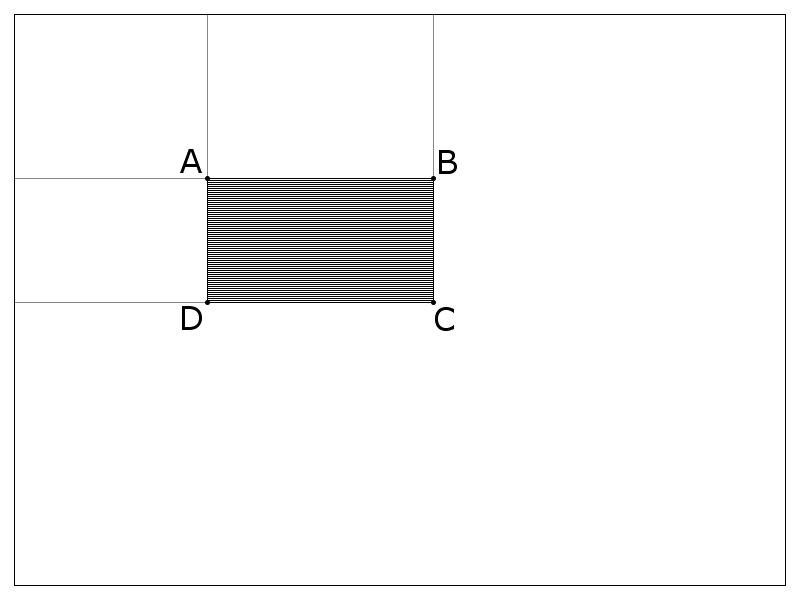
\includegraphics[width=30mm]{img/integral_image.png}}
  \caption{The sum of any rectangular region can be achieved by only three additions.}
\end{figure}


% Ukázka použití některých konstrukcí LateXu (odkomentujte, chcete-li)
% %%% Ukázka použití některých konstrukcí LaTeXu

\subsection{Ukázka \LaTeX{}u}
\label{ssec:ukazka}

This short subsection serves as an~example of basic \LaTeX{} constructs,
which can be useful for writing a~thesis.

Let us start with lists:

\begin{itemize}
\item The logo of Matfyz is displayed in figure~\ref{fig:mff}.
\item This is subsection~\ref{ssec:ukazka}.
\item Citing literature~\cite{lamport94}.
\end{itemize}

Different kinds of dashes:
red-black (short),
pages 16--22 (middle),
$45-44$ (minus),
and this is --- as you could have expected --- a~sentence-level dash,
which is the longest.
(Note that we have follwed \verb|a| by a~tilde instead of a~space
to avoid line breaks at that place.)

\newtheorem{theorem}{Theorem}
\newtheorem*{define}{Definition}	% Definice nečíslujeme, proto "*"

\begin{define}
A~{\sl Tree} is a connected graph with no cycles.
\end{define}

\begin{theorem}
This theorem is false.
\end{theorem}

\begin{proof}
False theorems do not have proofs.
\end{proof}

\begin{figure}
	\centering
	
\includegraphics[width=30mm]{../img/logo.eps}
	\caption{Logo of MFF UK}
	\label{fig:mff}
\end{figure}


\chapter*{Conclusion}
\addcontentsline{toc}{chapter}{Conclusion}

We have been testing our application on a Sony ST27i mobile device.
On the testing input data in Figure \ref{fig:input_samples} we obtained satisfiable results as is shown in Chapter \ref{chap:eval}.
For the testing input data, in the case of a bust of Ema Destinová we obtained a 3D model shaping the head and a part of a wall in the background.
In the second case, the input images gave us a result as an inclined plane in the angle of the memorial in the picture.
These results are comparable with the real appearance of the scenes and can be indicated as acceptable results.

Our implementation fails and does not give good results on noisy images or images of chaotic scenes.
In such a kind of scenes the features are matched incorrectly or is not even detected a sufficient number of SURF keypoints to reconstruct the 3D information. 
With high probability, the relative position of a pair of images of different illumination will not be estimated correctly.
Because of the relevant restriction on the area of the shape of an oriented rectangle where are the corresponding points searched (as we explained in Chapter \ref{chap:implementation}),
it is not possible to match the keypoints correctly when the registration fails.

\section*{Future work}

While we use a sum of absolute differences to detect the initial relative position, our approach fails on pairs of images with varying illumination.
Also it does not give good results on the images influenced by noise, which is quite common on the images taken by mobile phone camera, 
especially when the lightening conditions are not ideal.
This can be solved by obtaining the information of relative position by using mutual information while the mutual information is independent to the information of illuminance.

Current version of our program detects the  depth information from a pair of images.
Our implementation could be also extended to the input of $n$ photos. 
It would be necessary to find the relative position of all pairs of images.
This does not have to be calculated explicitly, but possibly we could estimate the position of two images when having the information about their position with the third image.
Detection and matching of SURF keypoints would be applied only to the pairs with an overlapping part.
Most of the implemented methods were designed to be easily extended for this purpose.

For a simple usage of the application we tried to implement an auto-capturing option for taking pictures.
However, we have not managed to optimalize it's behaviour, because it was not the main goal of this work. 
Therefore, it could be an option how to extend the application.
If we go even further, this way of using the device's equipment such an accelerometer can be used to estimate the relative position of taken pictures detected from the motion of the device.
We should note that we can not rely on any interaction with the user to calibrate the camera, since the the mobile phone lens causes a non-linear distortion of the image and non-linear distortion can not be modeled.






%%% Seznam použité literatury
%%% Seznam použité literatury je zpracován podle platných standardů. Povinnou citační
%%% normou pro bakalářskou práci je ISO 690. Jména časopisů lze uvádět zkráceně, ale jen
%%% v kodifikované podobě. Všechny použité zdroje a prameny musí být řádně citovány.

\def\bibname{Bibliography}
\begin{thebibliography}{99}
\addcontentsline{toc}{chapter}{\bibname}

\bibitem{cnnsynth}
  \emph{The 44\textsuperscript{th} President Inauguration.}
  CNN, Inc., 2013. Accessible from \url{http://www.cnn.com/themoment}, 2013.

\bibitem{surf2006}
  {\sc  H. Bay, A. Ess, T. Tuytelaars, and L. Van Gool.}
  \emph{Speeded–Up Robust Features (SURF).}
  In European Conference on Computer Vision, 2006.

\bibitem{ransac}
  {\sc M. A. Fischler and R. C. Bolles.} 
  \emph{Random sample consensus: A paradigm for model fitting with applications to image analysis and automated cartography.} 
  In Communications of the ACM, 1981.

\bibitem{harris1988}
  {\sc C. Harris and M. Stephens.} 
  \emph{A combined corner and edge detector.}
  In Proceedings of the Alvey Vision Conference, 1988.

\bibitem{multipleview}
  {\sc  R. Hartley and A. Zisserman.}
  \emph{Multiple View Geometry in Computer Vision.}
  Cambridge University Press, 2003.

\bibitem{hirschmuller2008}
  {\sc  H. Hirschmüller}
  \emph{Stereo Processing by Semiglobal Matching and Mutual Information.}
  In Pattern Analysis and Machine Intelligence, IEEE Transactions on, 2008.

\bibitem{marketshare}
  IDC Worldwide Mobile Phone Tracker, 2013.

\bibitem{siftsurf2009}
  {\sc L. Juan and O. Gwun.} 
  \emph{A Comparison of SIFT, PCA-SIFT and SURF.}
  In International Journal of Image Processing, 2009.

\bibitem{jurie2004}
  {\sc F. Jurie and C. Schmid.} 
  \emph{Scale–invariant shape features for recognition of object categories.}
  In Conference on Computer Vision and Pattern Recognition, 2004.

\bibitem{kadir2001}
  {\sc T. Kadir and M. Brady.} 
  \emph{Scale, saliency and image description.}
  In International Journal of Computer Vision, 2001.

\bibitem{siftsurf2001}
  {\sc N. Y. Khan, B. McCane, and G. Wyvill.} 
  \emph{SIFT and SURF Performance Evaluation Against Various Image Deformations on Benchmark Dataset.}
  In International Conference on Digital Image Computing: Techniques and Applications, 2001.

  
\bibitem{lindeberg1998}
  {\sc T. Lindeberg.} 
  \emph{Feature detection with automatic scale selection.}
  In International Journal of Computer Vision, 1998.

\bibitem{lowe1999}
  {\sc D. Lowe.} 
  \emph{Object recognition from scale–invariant features.}
  In CCV, 1999.

\bibitem{lucas}
  {\sc B. D. Lucas and T. Kanade. } 
  \emph{An iterative image registration technique with an application to stereo vision.}
  In Proceedings of Imaging Understanding Workshop, 1981.

\bibitem{roy1999}
  {\sc S. Roy.} 
  \emph{Stereo Without Epipolar Lines: A Maximum-Flow Formulation.}
  In International Journal of Computer Vision, 1999.

\bibitem{snavely2008}
  {\sc N. Snavely, R. Garg, S. M. Seitz, and R. Szeliski.} 
  \emph{Finding Paths through the World's Photos.}
  In Journal ACM Transactions on Graphics, 2008.

\bibitem{snavely2007}
  {\sc N. Snavely, S. M. Seitz, and R. Szeliski.} 
  \emph{Modeling the world from Internet photo collections.}
  In International Journal of Computer Vision, 2007.

\bibitem{snavely2006}
  {\sc N. Snavely, S. M. Seitz, and R. Szeliski.} 
  \emph{Photo tourism: Exploring photo collections in 3D.}
  In ACM Transactions on Graphics (SIGGRAPH Proceedings), 2006.

\bibitem{snavely2008}
  {\sc N. Snavely, S. M. Seitz, and R. Szeliski.} 
  \emph{Skeletal graphs for efficient structure from motion.}
  Computer Vision and Pattern Recognition, IEEE Conference on, 2008.

\bibitem{szeliski2010} 
  {\sc R. Szeliski.}
  \emph{Computer Vision: Algorithms and Applications.}
  Springer, 2010. 


\end{thebibliography}


%%% Tabulky v bakalářské práci, existují-li.
\chapwithtoc{List of Tables}

%%% Použité zkratky v bakalářské práci, existují-li, včetně jejich vysvětlení.
\chapwithtoc{List of Abbreviations}

%%% Přílohy k bakalářské práci, existují-li (různé dodatky jako výpisy programů,
%%% diagramy apod.). Každá příloha musí být alespoň jednou odkazována z vlastního
%%% textu práce. Přílohy se číslují.
\chapwithtoc{Attachments}

\openright
\end{document}
